\documentclass[xcolor=table]{beamer}

% \rowcolors{1}{gray!30}{gray!10}

\usetheme{Boadilla}
\usecolortheme{dolphin}
\useoutertheme[subsection=false]{smoothbars}

\setbeamercolor{frametitle}{fg = black, bg = white} 
\setbeamercolor{palette primary}{use=structure,fg=white,bg=structure.fg!60!white}
\setbeamercolor{palette secondary}{use=structure,fg=white,bg=structure.fg!90!white}
\setbeamercolor{palette tertiary}{use=structure,fg=white,bg=structure.fg!120!white}
\setbeamercolor{palette quaternary}{use=structure,fg=black,bg=white} %Top bar

\setbeamertemplate{enumerate subitem}[circle]%
\renewcommand{\insertsubenumlabel}{\alph{enumii}}

\usepackage{amsmath}
\usepackage{xcolor}
\usepackage{booktabs}
\usepackage[utf8]{inputenc}
\usepackage{hyperref}
\usepackage[table]{xcolor}
\definecolor{lightgray}{gray}{0.9}

\hypersetup{
    colorlinks,
    citecolor=blue,
    linkcolor=blue
}

\footnotesize \let\small\footnotesize

\author{Jonathan P. Latner, PhD}
\title{A/B test results}
\date{\today}

\beamertemplatenavigationsymbolsempty 
\setbeamerfont{page number in head/foot}{size=\tiny}
\setbeamertemplate{footline}[frame number]
\setbeamertemplate{caption}[numbered]
\setbeamertemplate{section in toc}[sections numbered]

\begin{document}

\section{Introduction}
\frame{\frametitle{ }
\titlepage
\thispagestyle{empty}
}

\subsection{}
\frame{\frametitle{Overview}
\begin{itemize}
    \item A/B test conducted during the month January, 2019
    \item Data are aggregated by treatment (2), days (31), and device (3)
    \item Total sample size 3.681.827 sessions (50/50 split)
    \item Results suggest:
    \begin{itemize}
        \item Small $+$ effect on conversion rate (n.s.)
        \item Small $-$ effect on revenues
        \item Suggests increase CR is result of cheaper purchases
        \item Effects are most visible on mobile users 
    \end{itemize}
\end{itemize}
}

\section{Aggregate}
\frame{\frametitle{Looking at the data} 

Q: Why do revenues have decimal places?  Is this in thousands?
\begin{table}[!h]
    \caption{}
    \begin{center}
    \resizebox{\textwidth}{!}{\begin{tabular}{lllrrrrrr}
 & treat & device & date & pageviews & uniqueviews & sessions & revenues & transactions \\
0 & Control & desktop & 20190101 & 90133.000000 & 65953 & 15615.000000 & 26516.199499 & 72.000000 \\
1 & Control & desktop & 20190102 & 149878.000000 & 108909 & 23030.000000 & 41575.678145 & 165.000000 \\
2 & Control & desktop & 20190103 & 153829.000000 & 112185 & 24470.000000 & 61002.022101 & 205.000000 \\
3 & Control & desktop & 20190104 & 154991.000000 & 111211 & 23480.000000 & 31768.423188 & 118.000000 \\
4 & Control & desktop & 20190105 & 119705.000000 & 87056 & 19381.000000 & 78505.386880 & 260.000000 \\
5 & Control & desktop & 20190106 & 134276.000000 & 96717 & 21133.000000 & 152900.387205 & 292.000000 \\
6 & Control & desktop & 20190107 & 113061.000000 & 83652 & 20294.000000 & 37037.681401 & 172.000000 \\
7 & Control & desktop & 20190108 & 103357.000000 & 77011 & 18123.000000 & 54678.632706 & 157.000000 \\
8 & Control & desktop & 20190109 & 102414.000000 & 76301 & 18984.000000 & 54674.876374 & 181.000000 \\
9 & Control & desktop & 20190110 & 93329.000000 & 70155 & 16927.000000 & 70416.784190 & 236.000000 \\
\end{tabular}
}
    \label{table_data_frame}
    \end{center}
\end{table}
}

\subsection{}
\frame{\frametitle{Aggregate totals by treatment group}

Values look similar by treatment group

\begin{figure}
    \caption{}
    \resizebox{\textwidth}{!}{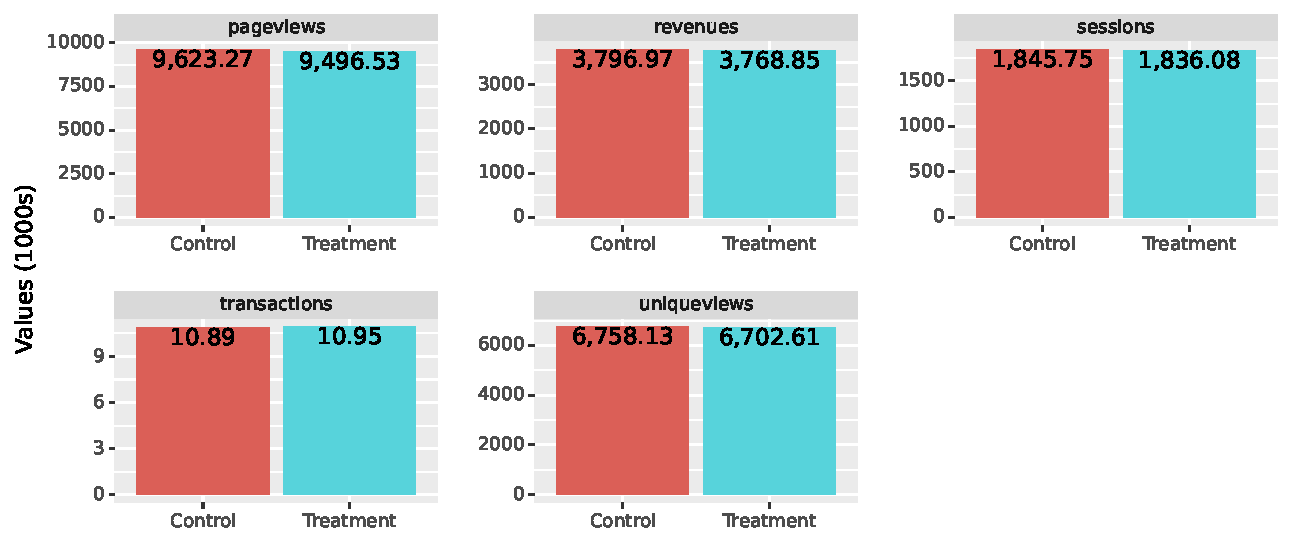
\includegraphics{../graphs/graph_values.pdf}}
    \label{graph_values}
\end{figure}
}

\subsection{}
\frame{\frametitle{Aggregate totals by treatment group and device}

Small differences are visible in revenues and transactions, by device category

\begin{figure}
    \caption{}
    \resizebox{\textwidth}{!}{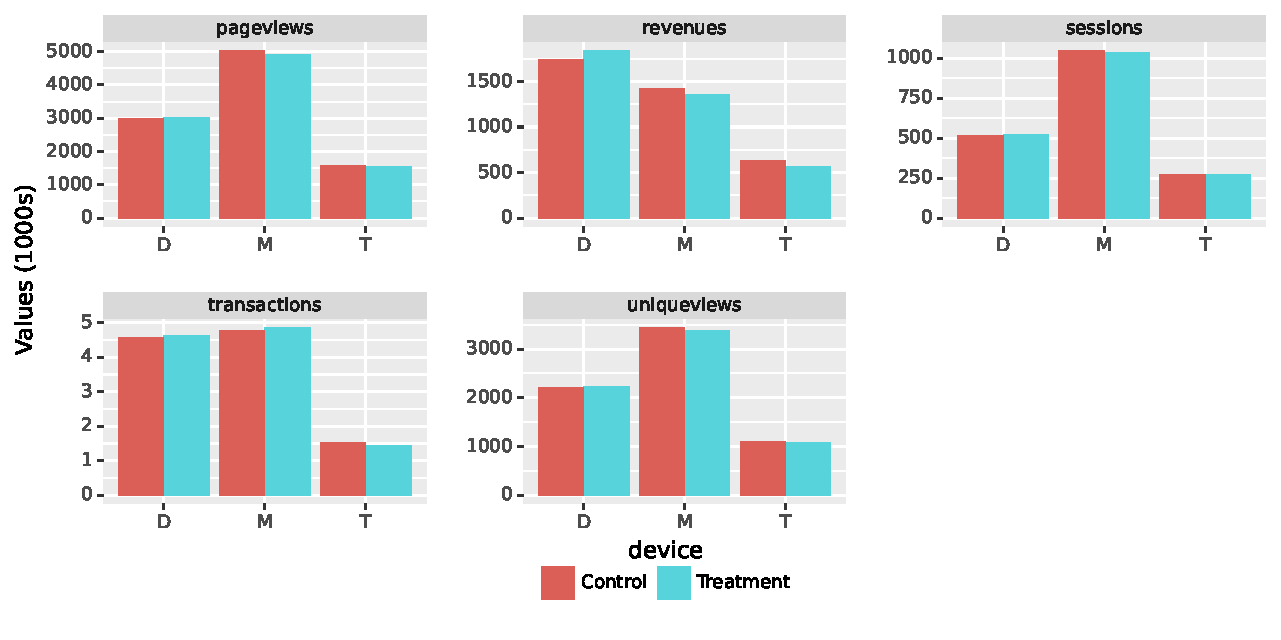
\includegraphics{../graphs/graph_values_device.pdf}}
    \label{graph_values_device}
\end{figure}
}

\subsection{}
\frame{\frametitle{Aggregate totals by treatment group and time}

General decline over time (as expected after December highs)

Small differences are visible in revenues and transactions


\begin{figure}
    \caption{}
    \resizebox{\textwidth}{!}{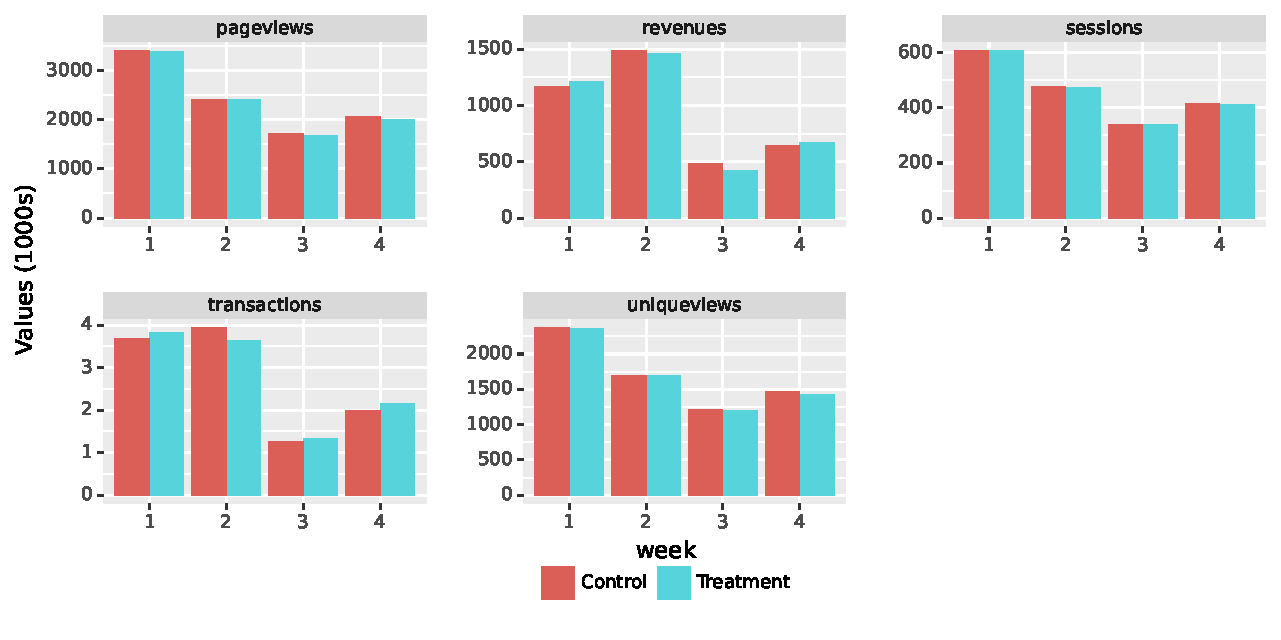
\includegraphics{../graphs/graph_values_time.pdf}}
    \label{graph_values_time}
\end{figure}
}

\section{Differences}
\frame{\frametitle{Effect of treatment group}

+ 0.61\% on transactions

Decline in all other variables

\begin{figure}
    \caption{}
    \vskip -5mm
    \resizebox{\textwidth}{!}{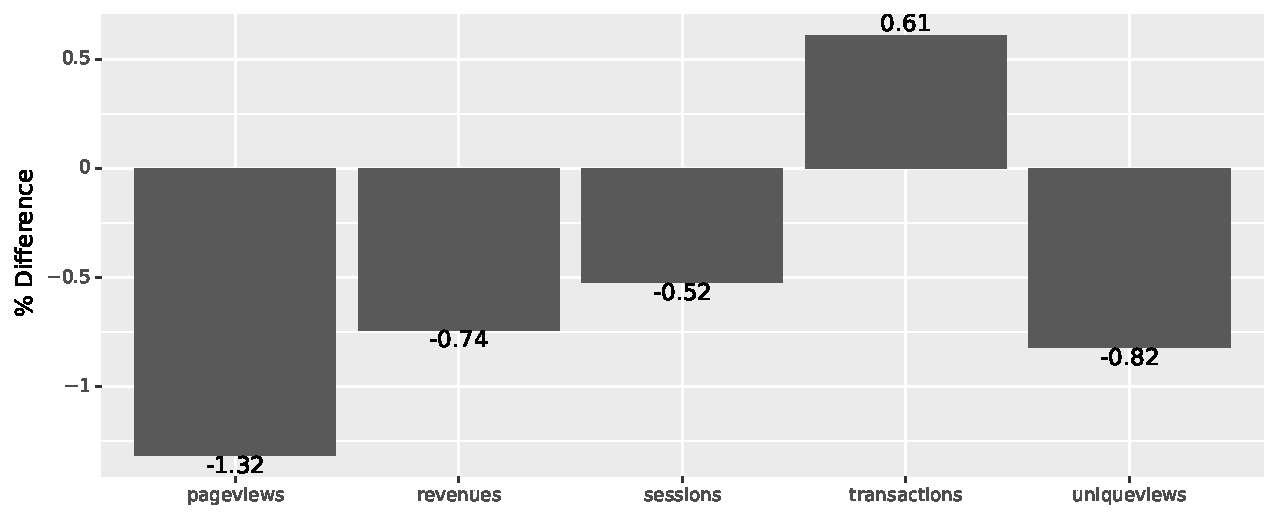
\includegraphics{../graphs/graph_diff.pdf}}
    \label{graph_diff}
\end{figure}
}


\subsection{}
\frame{\frametitle{Understanding differences by treatment group and device}

Effect is always positive among desktop users
Among mobile users, transactions are higher (but revenues lower)

\begin{figure}
    \caption{}
    \vskip -5mm
    \resizebox{\textwidth}{!}{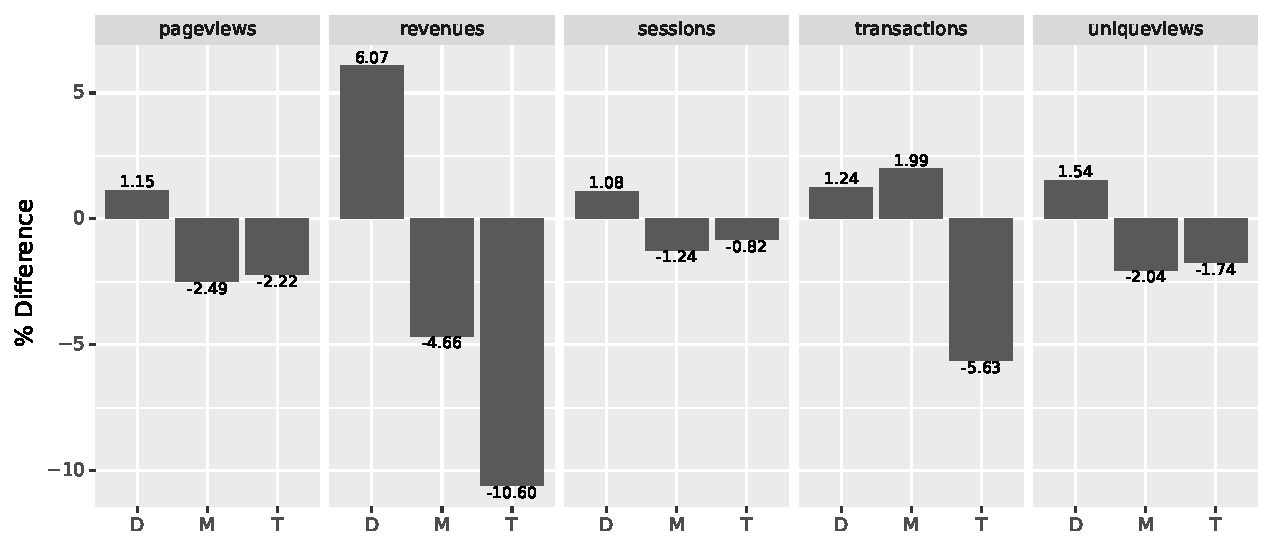
\includegraphics{../graphs/graph_diff_device.pdf}}
    \label{graph_diff_device}
\end{figure}
}

\subsection{}
\frame{\frametitle{Understanding differences by treatment group and time}

Mixed effect of treatment over time

Transactions are positive (except week 2)

In week 3, revenues are really negative 

\begin{figure}
    \caption{}
    \vskip -5mm
    \resizebox{\textwidth}{!}{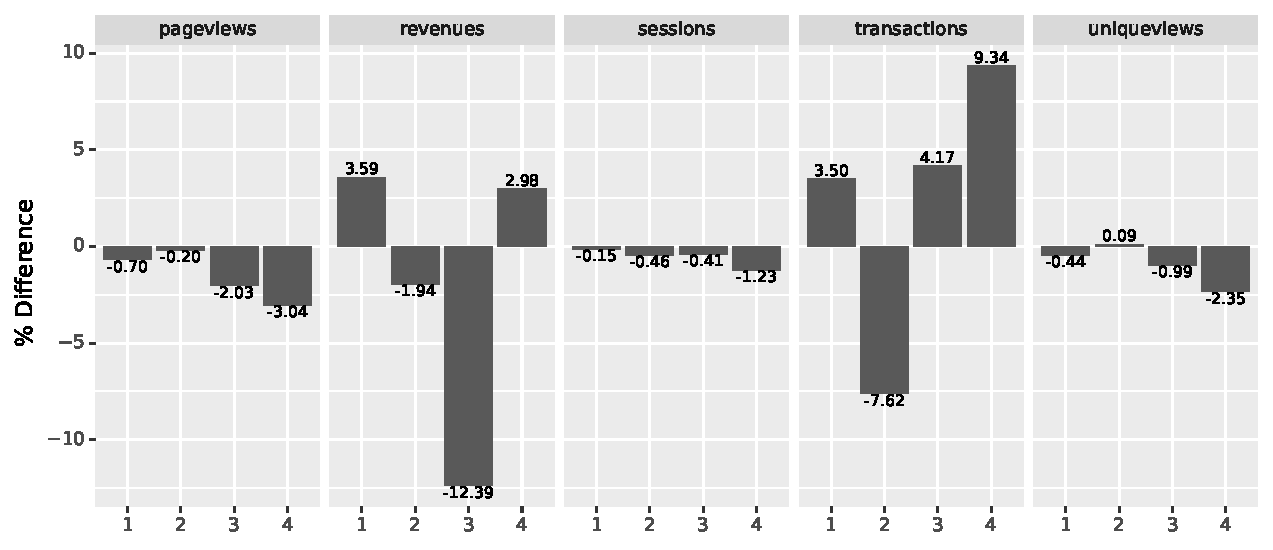
\includegraphics{../graphs/graph_diff_time.pdf}}
    \label{graph_diff_time}
\end{figure}
}

\section{CR}
\frame{\frametitle{Effect of treatment on conversion rate (CR)}

conversion rate (CR) = transactions/sessions

Small positive effect (+0.007 or 1.4\%), but not significant

To achieve significance, we need 9.284.592 sessions (i.e. 4 more  months)

\begin{figure}
    \caption{}
    \vskip -5mm
    \resizebox{\textwidth}{!}{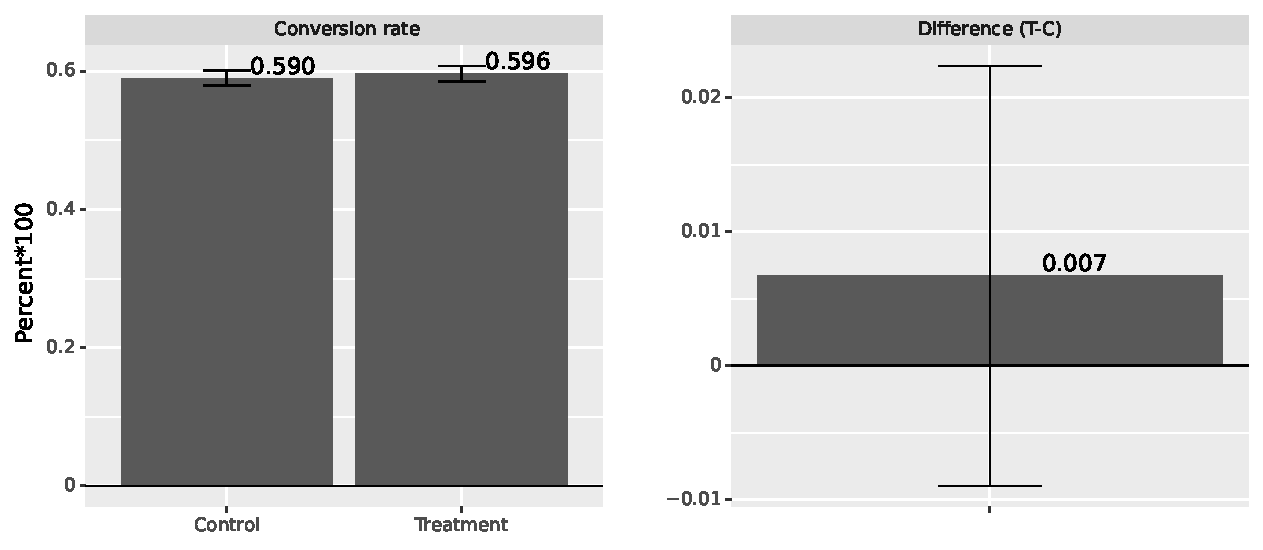
\includegraphics{../graphs/graph_cr.pdf}}
    \label{graph_cr}
\end{figure}
}

\frame{\frametitle{Conversion rate by device}

In mobile users, small positive effect (+0.015 or 3.3\%), but not significant

To achieve significance, we would need 1.796.940 mobile sessions ($<$ 1 more month) 


\begin{figure}
    \caption{}
    \vskip -10mm
    \resizebox{\textwidth}{!}{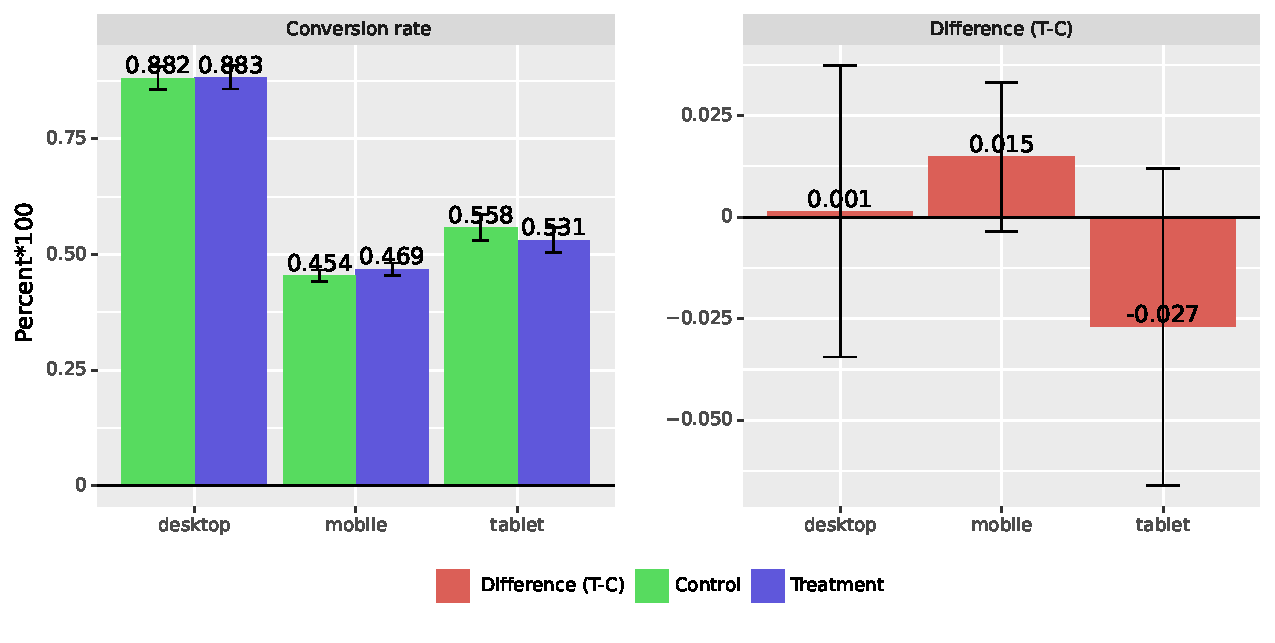
\includegraphics{../graphs/graph_cr_device.pdf}}
    \label{graph_cr}
\end{figure}
}



\section{Conclusion}
\frame{\frametitle{Conclusions}
\begin{itemize}
    \item Effect of test on CR is positive, but not significant
    \begin{itemize}
        \item Total effect could be significant with more time (4 more months)
        \item Effect is most positive on mobile users
    \end{itemize}
    \item But don't forget about revenues
    \begin{itemize}
        \item Treatment group has 30.000 or 0.5\% lower revenues
        \item If we extended the test, revenues could decline by 150.000
        \item In mobile users, treatment reduces revenues by 4.6\% 
    \end{itemize}
    \item Recommendation
    \begin{itemize}
        \item Look for other treatments that are more effective
        \item Focus on effect of treatment on mobile users
    \end{itemize}
\end{itemize}
}

\frame[c]{\frametitle{}
\centering
Thank you\\\
}



\end{document}


